\documentclass[11pt,fleqn]{exam}
\usepackage[utf8]{inputenc}

\usepackage[margin=1in]{geometry}
\usepackage{amsmath,amssymb}
\usepackage{gensymb}
\usepackage{multicol}
\usepackage{float}
\usepackage{graphicx}
\usepackage{units,icomma}
\usepackage[bahasa]{babel}
\usepackage[colorlinks,linkcolor=blue,urlcolor=blue]{hyperref}
\usepackage[margin=1.5cm]{caption}
\usepackage{wasysym}
\usepackage[shortlabels]{enumitem}

\hyphenation{
  chro-no-ampe-ro-met-ric
  ber-dia-me-ter
  de-ngan
  meng-alam-i
  me-nem-pati
  mic-ro-graphs
  man-hat-tan-henge}

\addto\extrasbahasa{
	\def\figureautorefname{Gambar}
}

\renewcommand{\figurename}{Gambar.}
\def\equationautorefname{Persamaan}
\newcommand{\class}{OLIMPIADE ASTRONOMI}
\newcommand{\term}{Tingkat Provinsi - 2018}
\newcommand{\examnum}{OSP Astronomi 2018}
%\newcommand{\examdate}{11/02/2014}
%\newcommand{\timelimit}{120 Minutes}

\pagestyle{head}
\firstpageheader{}{}{}
\runningheader{\examnum}{}{Halaman \thepage\ dari \numpages}
\runningheadrule


\begin{document}

\noindent
\begin{tabular*}{\textwidth}{l @{\extracolsep{\fill}} r @{\extracolsep{6pt}} l}
\textbf{\class} \\% & \textbf{Name:} & \makebox[2in]{\hrulefill}\\
\textbf{\term}  %&&\\
%\textbf{\examnum} &&\\
%\textbf{\examdate} &&\\
%\textbf{Time Limit: \timelimit} & Teaching Assistant & \makebox[2in]{\hrulefill}
\end{tabular*}\\
\rule[2ex]{\textwidth}{2pt}

\noindent
\begin{tabular}{ll}
Copyright (c) 2018 & Ridlo W. Wibowo (ridlo.w.wibowo@gmail.com)\\
                   & Sulistiyowati (sulis.astro08@gmail.com)
\end{tabular}

\vspace{0.3cm}
\noindent
Solusi ini dibuat tanpa jaminan kesesuaian dengan solusi resmi dari juri olimpiade sains bidang Astronomi. Pengguna boleh menyebarluaskan dan/atau memodifikasi solusi ini dengan mencantumkan sumber asli. Hak cipta soal ada pada Kemendiknas dan dilindungi undang-undang.

\vspace{0.4cm}
\noindent
\rule[2ex]{\textwidth}{1.5pt}

\textbf{Soal Pilihan Ganda}

\begin{questions}
\question Convection can occur inside a star. This stellar convection describes motion of gas. If we consider a star as an ideal gas. Choose the right statement representing stellar convection in which a packet of gas rises slightly
\begin{choices}
\choice The gas cools to a lower temperature than its new surroundings, so that it has a higher density than surroundings, it will continue to rise.
\choice The temperature gradient of the gas is steep enough and the density is less dense than its new surroundings, then the gas will sink back again.
\choice The gas cools to a lower temperature than its new surroundings, but its density is the same with surroundings. This makes the gas continues to rise.
\choice If the temperature gradient of the gas is steep enough, the gas is less dense than its new surroundings, and it will continue to rise.
\choice The gas has higher temperature and higher density than surroundings, so it will sink back again to where it comes from.
\end{choices}

\textit{Jawaban: }D\\
Convection is one way to transport energy/heat in a star by rising and falling of gas elements. The main idea is hot gas from deeper part of a star will have less density and move upward closer to the star's surface, transporting its energy/heat to the surrounding. After that, the gas cools, gets denser and sinks downward. The gas then acquires energy from around the center of the star and the process occurs again repetitively.

A little bit more detailed explanation is the following. When a blob of hot gas from a deeper part of the star is rising slightly upward, the gas will find itself in a new environment. In a star, it is expected that the further from the center, the lower the temperature and pressure there is.  Since the gas blob is now in a lower pressure environment, it will expand and cool. If the temperature gradient is steep, i.e. the surrounding temperature drops more than the hot blob of gas, then the gas blob's density will be less dense than the surrounding, since the gas is still hotter than its environment. Therefore the gas blob will continue to rise. The process keeps going on until the gas transfers its energy to its environment and gets cooler, denser than its surrounding. In that case, the gas blob will then sink back downward. Taking energy again from hot environment near the center of the star.

Hence, the correct answer for the question is D.

\vspace{1.5cm}
\question Sebuah bintang, yang mempunyai massa 10$M_{\odot}$, radius 10$R_{\odot}$, dan periode rotasi 3 bulan, mengalami keruntuhan menjadi suatu bintang neutron dengan radius 10 km. Asumsikan bintang berbentuk bola. Kecepatan rotasi bintang neutron yang terbentuk adalah
\begin{choices}
\choice $3,5\times 10^3$ km/detik
\choice $1,9\times 10^{15}$ km/detik
\choice $3,8\times 10^{17}$ km/detik
\choice $1,6\times 10^7$ km/detik
\choice $3,9\times 10^6$ km/detik
\end{choices}

\textit{Jawaban: }E\\
Dalam proses ini dapat kita asumsikan besar (dan arah) momentum sudut bintang tetap/kekal, sebelum mengalami keruntuhan (indeks $i$) dan setelahnya (indeks $f$),
\begin{eqnarray*}
L_i & = & L_f\\
I_i\omega_i & = & I_f\omega_f\\
\end{eqnarray*}
Dengan asumsi bola pejal dan rotasi seperti benda tegar, berlaku:
\begin{eqnarray*}
\frac{2}{5}M_iR_i^2\frac{v_i}{R_i} & = & \frac{2}{5}M_fR_f^2\frac{v_f}{R_f}\\
\end{eqnarray*}
Massa bintang tidak berubah sehingga $M_i=M_f$.
\begin{eqnarray*}
R_iv_i&=&R_fv_f\\
v_f&=&\frac{R_i}{R_f}v_i\\
v_f&=&\frac{R_i}{R_f}\frac{2\pi R_i}{P_i}\\
v_f&=&3,91\times 10^6\text{  km/detik}
\end{eqnarray*}
Jadi, jawaban yang paling tepat adalah E. 

Catatan: jangan lupa mengubah satuan pada data yang diketahui ke satuan yang sesuai.

\question Hasil pengamatan menyimpulkan bahwa alam semesta mengembang. Hal ini diperoleh dari pengamatan
\begin{choices}
\choice Gelombang gravitasi dari materi gelap.
\choice Gugus bola di Galaksi Bima Sakti bergerak mengelilingi pusat galaksi.
\choice Pergeseran merah dari supernova SN Ia.
\choice Pergeseran merah dari bintang-bintang di tepi lengan spiral Bima Sakti.
\choice Pergeseran merah dari eksoplanet di Galaksi Bima Sakti.
\end{choices}

\textit{Jawaban: }C\\
Bukti alam semesta mengembang mulanya diperoleh dari hasil pengamatan Edwin Hubble terhadap spektrum galaksi-galaksi pada awal abad ke-20. Lebih dari setengah abad kemudian, Saul Perlmutter, Brian Schmidt, dan Adam Riess, beserta tim mereka, mengolah data supernova tipe Ia. Hasil mereka mengindikasikan bahwa alam semesta mengembang dipercepat. Maka jawaban yang paling tepat di antara pilihan yang tersedia yakni C.

\question \textit{Manhattanhenge} adalah sebuah nama yang diberikan pada peristiwa sebelum tenggelam dan setelah terbit Matahari yang terjadi empat kali dalam setahun (dua kali untuk terbenam dan dua kali untuk terbit), yaitu saat posisi Matahari tepat sejajar arah timur-barat jalan-jalan utama kota New York, Amerika Serikat (lihat gambar di bawah ini). Salah satu peristiwa \textit{Manhattanhenge} tahun ini terjadi saat menjelang Matahari tenggelam pada tanggal 11 Juli. Selain tanggal 11 Juli, kapan \textit{Manhattanhenge} dapat terjadi lagi?
\begin{figure}[H]
\centering
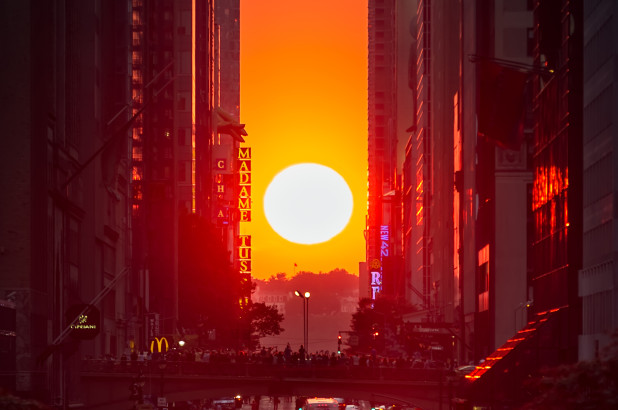
\includegraphics[scale=0.4]{manhattanhenge.jpg}
\caption{Sumber gambar nypost.com}
\end{figure}
\begin{choices}
\choice 30 Mei
\choice 30 Juni
\choice 31 Juli
\choice 11 Desember
\choice 11 Januari
\end{choices}

\textit{Jawaban: }A

Berdasarkan informasi tanggal di soal, dapat disimpulkan bahwa jalan-jalan utama di New York membentang sedikit melenceng dari arah tepat timur barat. Jika jalanannya tepat sejajar arah timur-barat, maka peristiwa ini hanya mungkin terjadi saat Matahari ada di ekuator (20 Maret dan 23 September).

\textit{Manhattanhenge} terjadi ketika Matahari tampak di ujung jalan-jalan utama di New York sesaat setelah terbit dan sebelum terbenam, artinya azimut terbit/tenggelam Matahari sama dengan arah jalan utama di sana. Lihat sketsa pada \autoref{manhattan} berikut.
\begin{figure}[H]
\centering
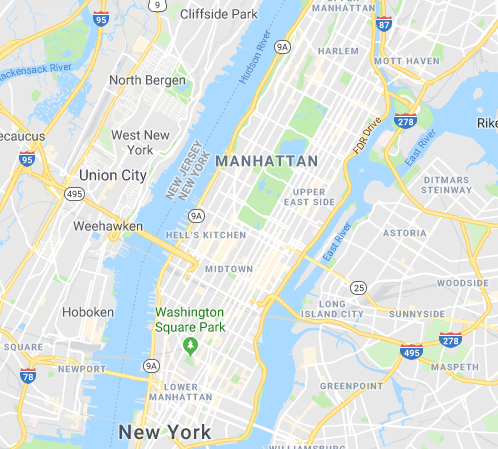
\includegraphics[width=0.39\textwidth]{manhattan.png}
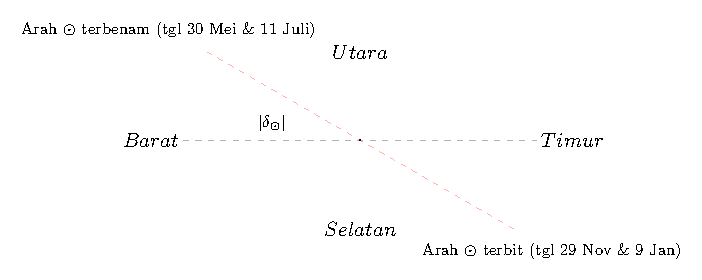
\includegraphics[width=0.6\textwidth]{manhattanhenge.pdf}
\caption{(Kiri) Peta kota Manhattan yang menunjukkan arah jalan-jalan utamanya. (Kanan) Sketsa posisi Matahari saat terbit dan terbenam pada peristiwa \textit{Manhattanhenge}. Garis putus-putus merah menunjukkan arah jalan-jalan utama (bukan gerak harian Matahari \smiley{}).}
\label{manhattan}
\end{figure}

Pada momen-momen tersebut nilai deklinasi Matahari haruslah tertentu sehingga ketika terbenam posisi azimutnya ($\cos{A} = \frac{\sin{\delta_{\odot}}}{\cos{\phi}}$) yang sesuai dengan arah jalan di sana. Pada tanggal 11 Juli, dengan $t$ jumlah hari yang terlampaui sejak tanggal 20 Maret, kita bisa hitung deklinasi Matahari ketika terjadi \textit{Manhattanhenge}.
\begin{eqnarray*}
\delta_{\odot}&=&23,5\text{\degree}\sin (\frac{t}{365,25}360\text{\degree})\\
\delta_{\odot}&=&22,03\text{\degree}
\end{eqnarray*}

Dengan menghitung persamaan di atas untuk nilai $t$ lain yang memenuhi, Matahari akan memiliki deklinasi sebesar itu pada tanggal: 30 Mei (Matahari di utara, peristiwa \textit{Manhattanhenge}-terbenam). Sedangkan untuk peristiwa \textit{Manhattanhenge}-terbit akan terjadi pada tanggal 29 November dan 9 Januari (Matahari di selatan). Simetri fungsi sinusoidal dapat dimanfaatkan untuk mencari tanggal-tanggal tersebut dengan mudah. Jadi, jawaban yang tepat adalah A.



\question Pilihlah pernyataan yang SALAH di bawah ini:
\begin{choices}
\choice Bintang dapat runtuh dalam hitungan beberapa menit.
\choice Bintang dapat menghabiskan energi panas (termal) dalam beberapa jam.
\choice Bintang dapat melakukan reaksi fusi nuklir selama milyaran tahun.
\choice Bintang dapat bermassa puluhan kali massa Matahari.
\choice Temperatur bintang dapat menurun dari pusat hingga fotosfer, lalu meningkat kembali ke arah korona bintang.
\end{choices}

\textit{Jawaban: }B\\
Evaluasi pernyataan A:\\
Runtuhnya bintang sebagai akibat gravitasi dirinya dengan menganggap tiba-tiba tidak ada tekanan penahan gravitasi terjadi dalam skala waktu dinamik. Skala waktu dinamik terjadi dalam orde menit.
\begin{equation*}
t_d = \frac{\pi}{8} \sqrt{\frac{R^3}{GM}}
\end{equation*}
Pernyataan A benar.

Evaluasi pernyataan B:\\
Jika reaksi nuklir berhenti, maka bintang tidak akan langsung berhenti bersinar. Bintang masih akan bersinar dengan menghabiskan energi ikat gravitasinya. Jika ini terjadi, tekanan tidak akan serta merta hilang secara tiba-tiba, melainkan bertahap seiring lolosnya foton dari bintang. Skala waktu yang relevan dengan proses ini dinamakan skala waktu termal (Kelvin-Helmholtz) yang besarnya untuk Matahari dalam orde puluhan juta tahun.
\begin{equation*}
t_t \approx \frac{0,5 G M^2 / R}{L}
\end{equation*}

\textbf{Pernyataan B salah.}

Evaluasi pernyataan C:\\
Waktu yang diperlukan untuk menghabiskan energi hasil reaksi nuklir di pusat bintang dinamakan skala waktu nuklir. Reaksi fusi di dalam bintang dapat terjadi selama milyaran tahun.
\begin{equation*}
t_n \approx \frac{0,007 \cdot 0,1 \cdot M c^2}{L}
\end{equation*}
Pernyataan C benar.

Evaluasi pernyataan D:\\
Rentang massa bintang yang diketahui ada dan mengalami reaksi fusi di pusatnya adalah antara 0,9 massa Matahari hingga ratusan massa Matahari. Secara teori mungkin dari $\sim 0,1M_{\odot}$ hingga $\sim 150 M_{\odot}$ \\
Pernyataan D benar.

Evaluasi pernyataan E:\\
Temperatur tertinggi bintang ada di pusat, kemudian menurun ke arah permukaan. Temperatur korona meningkat, lebih tinggi daripada fotosfer bintang.\\
Pernyataan E benar.


\question Diketahui gugus bintang Pleiades memiliki anggota sebagai berikut
\begin{table}[h!]
\centering
\begin{tabular}{|c|c|c|c|}
\hline
TYC2 & RAJ2000 & DEJ2000 & Paralaks\\
     & (jam menit detik) & (\degree \hspace{0.5cm}'\hspace{0.5cm} '') & (mili detik busur)\\
\hline
1800-1974-1 & 03 46 13,7616 & +24 11 47,623 & 7,56\\
\hline
1800-1908-1 & 03 46 27,3010 & +24 15 17,326 & 7,74\\
\hline
1800-1935-1 & 03 47 10,0757 & +24 16 35,278 & 7,15\\
\hline
1800-1579-1 & 03 47 04,2364 & +23 59 42,092 & 7,13\\
\hline
1800-2201-1 & 03 47 21,0609 & +24 06 57,888 & 7,88\\
\hline
1800-1607-1 & 03 47 19,3667 & +24 08 20,157 & 7,64\\
\hline
\end{tabular}
\end{table}

Simpangan baku (standar deviasi) jarak bintang-bintang di gugus tersebut adalah
\begin{choices}
\choice 133,23 pc
\choice 155,93 pc
\choice 5,58 pc
\choice 7,52 pc
\choice 0,31 pc
\end{choices}

\textit{Jawaban: }C\\
Jarak bintang dan paralaks terhubung melalui persamaan: $d=\frac{1}{p}$, dengan $d$ dalam parsek dan $p$ dalam detik busur.

\begin{table}[h!]
\centering
\begin{tabular}{cccc}
\hline
\\[-1em]
$i$ & $p_i$ & $d_i$ & $(d_i-\overline{d})^2$\\
 Bintang ke -     & (mili detik busur) & parsek\\
\hline
1 & 7,56 & 132,275 & 0,912 \\
2 & 7,74 & 129,199 & 16,250 \\
3 & 7,15 & 139,860 & 43,958 \\
4 & 7,13 & 140,252 & 49,314 \\
5 & 7,88 & 126,904 & 40,025 \\
6 & 7,64 & 130,890 & 5,476 \\
\hline
\\[-1em]
  &  & $\overline{d}=133,230$ & $\Sigma(d_i-\overline{d})^2=155,934$
\end{tabular}
\end{table}

Standar deviasi untuk sampel bintang anggota gugus di atas:
$$stdev=\sqrt{\frac{\Sigma(d_i-\overline{d})^2}{N-1}}=5,585$$ 
maka jawaban paling tepat adalah C.

\question Apa yang akan terjadi jika pembakaran termonuklir di inti Matahari tiba-tiba berhenti?
\begin{choices}
\choice Matahari akan langsung padam dan tidak bersinar lagi karena sumber energinya berhenti diproduksi.
\choice Matahari masih akan tetap bersinar karena masih ada energi gravitasi akibat intinya yang mengerut.
\choice Inti Matahari akan langsung meledak karena tekanan yang tiba-tiba dari permukaannya.
\choice Lapisan permukaan Matahari akan langsung mengembang menjadi bintang raksasa.
\choice Matahari akan tetap bersinar karena sumber utama energi Matahari bukan dari inti, namun dari lapisan permukaannya.
\end{choices}

\textit{Jawaban: }B\\
Baca penjelasan pada soal nomor 5.

\question Pada tahun 1582, kalender Masehi mengalami reformasi, dan kemudian dinamakan kalendar Gregorian. Dengan menggunakan periode sinodis Bulan dari daftar konstanta, jumlah bulan purnama selama 5700000 tahun Gregorian adalah sebanyak
\begin{choices}
\choice 70550000
\choice 70500000
\choice 70499151
\choice 69500218
\choice 68400000
\end{choices}

\textit{Jawaban: }C

Satu tahun Gregorian: $T_G=365,2425$ hari. 

Satu periode sinodis Bulan: $T_{Syn}=29,5306$ hari.

Jumlah Bulan purnama selama $N$ tahun Gregorian: 
$$N_{\text{purnama}}= \frac{N \cdot T_G}{T_{Syn}}$$ 
Maka, selama 5700000 tahun Gregorian, jumlah Bulan purnama $=70499151,727$ (bulatkan ke bawah karena yang ditanya jumlah kejadian purnama).

Jadi, jawaban yang paling tepat C.

\question Berikut ini pernyataan yang SALAH terkait pemanasan debu antar bintang adalah
\begin{choices}
\choice Debu antar bintang menyerap energi dari cahaya bintang.
\choice Debu antar bintang mendapat energi dari tumbukan dengan atom dan partikel debu lainnya.
\choice Debu antar bintang menyerap energi dari sublimasi atom atau molekul di permukaan debu.
\choice Debu antar bintang menyerap energi dari gelombang kejut akibat ledakan supernova.
\choice Debu antar bintang menyerap energi dari reaksi kimia yang terjadi di permukaan debu.
\end{choices}

\textit{Jawaban: }C\\
Debu antar bintang dapat mengalami pemanasan dengan menyerap energi dari:
\begin{itemize}
\item Sinar kosmik berenergi rendah, serta sinar X.
\item Sinar UV dari bintang panas.
\item Energi yang dihasilkan oleh reaksi pembentukan molekul H\textsubscript{2} dari atom-atom H di permukaan debu.
\item Tumbukan dengan atom atau partikel debu lain.
\item Keruntuhan gravitasi awan debu antar bintang.
\item Ledakan supernova.
\item Angin bintang.
\item Pengembangan daerah HII.
\item Gelombang kejut magnetohidrodinamik dari sisa supernova.
\end{itemize}

Untuk soal berikut ini, jawablah
\begin{choices}
\choice jika 1, 2, dan 3 benar
\choice jika 1 dan 3 benar
\choice jika 2 dan 4 benar
\choice jika 4 saja benar
\choice jika semua benar
\end{choices}

\question Stellar mass determines stellar evolution. Scientists classify stellar mass into three categories, i.e. low mass stars, intermediate-mass stars, and high-mass stars. Choose the right statement(s) below that corresponds to the evolution of single stars.
\begin{enumerate}
\item High-mass stars have short lives, becoming hot enough to make iron, and end in nova explosions.
\item Stars of higher mass have higher core temperature and more rapid fusion, making those stars more luminous.
\item Low-mass stars have long lives, becoming hot enough to fuse carbon nuclei, and end as white dwarfs.
\item Intermediate-mass stars can make elements heavier than carbon and end as white dwarfs.
\end{enumerate}

\textit{Jawaban: }C\\
Statement 1. ``High-mass stars have short lives, becoming hot enough to make iron, and end in nova explosions."\\
High-mass stars end in supernova explosions.\\
Statement 1 is not correct.\\
Statement 2. ``Stars of higher mass have higher core temperature and more rapid fusion, making those stars more luminous."\\
\textbf{Statement 2 is correct.}\\
Statement 3. `` Low-mass stars have long lives, becoming hot enough to fuse carbon nuclei, and end as white dwarfs."\\
Low-mass stars can not be hot enough to fuse carbon nuclei. They cease fusing after carbon nuclei core is formed, and end as white dwarfs.\\
Statement 3 is not correct.\\
Statement 4. ``Intermediate-mass stars can make elements heavier than carbon and end as white dwarfs."\\
\textbf{Statement 4 is correct.}\\
Hence, statements 2 and 4 are correct, the answer is C.


\vspace{0.5cm}
\textbf{Soal Isian Singkat}

\question Diketahui spektrum galaksi sebagai berikut.
\begin{figure}[h!]
\centering
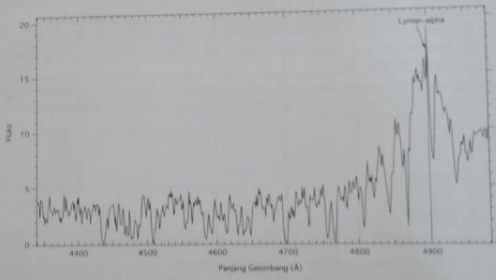
\includegraphics[scale=1]{spektrumgalaksi.PNG}
\end{figure}

Deret Lyman mengikuti persamaan
\begin{equation*}
\frac{1}{\lambda}=R(1-\frac{1}{n^2})
\end{equation*}

dengan konstanta Rydberg $R=1,0968\times 10^7$ m\textsuperscript{-1} dan $n=2,3,4,$\ldots dan seterusnya. Berdasarkan spektrum galaksi di atas, pergeseran merah (\textit{redshift}) dari galaksi tersebut adalah \ldots.

\textit{Jawaban: } 3,031

Garis Lyman alpha dihitung untuk $n$ bernilai 2. Maka panjang gelombang diam garis Lyman alpha seharusnya: 
\begin{eqnarray*}
\frac{1}{\lambda_0} &=& R(1-\frac{1}{2^2})\\
\lambda_0 &=& 1215,658 \text{  \AA}
\end{eqnarray*}
Dalam gambar tersebut, garis Lyman alpha teramati bergeser hingga panjang gelombang $\lambda=4900$ angstrom. Maka, \textit{redshift} ($z$) garis Lyman alpha galaksi tersebut adalah sebesar 
$$z=\frac{\lambda-\lambda_0}{\lambda_0}=3,031$$

\question Diketahui tekanan atmosfer pada permukaan Bumi adalah $1,0\times 10^5$ kg m\textsuperscript{-1} s\textsuperscript{-2} dan 70\% permukaan Bumi tertutupi air laut dengan kedalaman rata-rata 4267 m. Massa jenis air laut adalah 1025 kg m\textsuperscript{-3}. Jika air laut di Bumi seluruhnya menguap ke atmosfer, maka tekanan atmosfer di Bumi yang baru adalah \ldots\ldots kg m\textsuperscript{-1} s\textsuperscript{-2}.

\textit{Jawaban: } $3,006\times 10^7$

Konstanta gravitasi universal $G=6,673\times 10^{-11}$ m$^3$/kg/s$^2$.\\
Jari-jari Bumi $R_{\oplus}=6378$ km.\\
Massa Bumi $M_{\oplus}=5,97\times 10^{24}$ kg.\\
Tekanan atmosfer di permukaan Bumi muncul dari gaya berat atmosfer yang melingkupi Bumi, yang disangga oleh luas permukaan bola Bumi. Jika volum air laut $V_{sea}$, volum Bumi $V_{\oplus}$, dan volum Bumi yang terlingkupi radius pada kedalaman $h=4267$ m adalah $V_{R_{\oplus-}}$, maka:
\begin{eqnarray*}
V_{sea}&=&70\%(V_{\oplus}-V_{R_{\oplus-}})\\
&=&0,7(\frac{4}{3}\pi R_{\oplus}^3-\frac{4}{3}\pi (R_{\oplus}-h)^3)\\
&=&0,7\frac{4}{3}\pi(R_{\oplus}^3-(R_{\oplus}-h)^3)\\
&=&1,526\times 10^{18} \text{ m$^3$}
\end{eqnarray*}

Massa air laut yang menguap: $m_{sea}=\rho_{sea}V_{sea}=1,564\times 10^{21}$ kg.

Dengan $A_{\oplus}$ menyatakan luas permukaan Bumi dan $g$ percepatan gravitasi Bumi, tekanan tambahan yang muncul akibat menguapnya air laut:
\begin{eqnarray*}
P_{add}&=&\frac{m_{sea}g}{A_{\oplus}}\\
&=&\frac{m_{sea}\frac{GM{\oplus}}{R_{\oplus}^2}}{4\pi R_{\oplus}^2}\\
&=&\frac{GM_{\oplus}m_{sea}}{4\pi R_{\oplus}^4}\\
&=&2,996\times 10^7 \text{ kg m$^{-1}$ s$^{-2}$}
\end{eqnarray*}
Tekanan atmosfer baru di permukaan Bumi: $P_{baru}=P_{atm}+P_{add}=1\times 10^5+2,996\times 10^7=3,006\times 10^7$  kg m$^{-1}$ s$^{-2}$.

\question Jika pada saat gerhana bulan perigee (atau istilah populernya \textit{supermoon}), jarak Bumi-Bulan adalah 363300 km, dan pada saat gerhana bulan apogee (\textit{micromoon}), jarak Bumi-Bulan adalah 405500 km. Perbandingan gaya pasang surut (gaya tidal) antara peristiwa gerhana bulan perigee dengan gerhana bulan apogee tersebut adalah \ldots.

\textit{Jawaban: }1,391\\
Gaya pasang surut nilainya berbanding terbalik dengan pangkat tiga jarak ($\propto \frac{1}{d^3}$). Maka, perbandingan gaya pasang surut saat perigee dan apogee: 
$$\frac{F_{\text{tidal, peri}}}{F_\text{tidal, apo}} = \left( \frac{d_{\text{apo}}}{d_{\text{peri}}} \right)^{3}=1,391$$

\question Gugus bintang Messier 6 (\textit{Butterfly Cluster}) memiliki diameter sudut 20'. Jika objek tersebut diamati dengan deterktor \textit{Charge Couple Device} (CCD) berukuran 510$\times$510 piksel\textsuperscript{2} (1 piksel = 9 mikron), maka panjang fokus teleskop yang digunakan untuk dapat mengamati keseluruhan objek adalah \ldots m.

\textit{Jawaban: } 0,789

Berdasarkan informasi pada soal, jika seluruh area CCD digunakan untuk tepat mengamati gugus M6, maka ukuran linier bayangan: 

$D = 510$ piksel $\times$ 9 mikron $=4590$ mikron $=4,59\times 10^{-3}$ m.

Secara geometri (lihat \autoref{fig:telescopeAndCCD}), berlaku 

$D = F \tan{\alpha}$, 

dengan $F$ menyatakan panjang fokus teleskop dan $\alpha$ diameter sudut objek. Maka panjang fokus teleskop yang digunakan apabila dipasangkan dengan CCD tersebut haruslah $F \leq 0,789$ meter.
\begin{figure}[H]
\centering
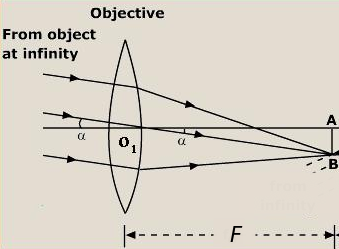
\includegraphics[width=0.5\textwidth]{telescope.png}
\caption{Bayangan yang terbentuk di fokus objektif yang ditangkap oleh CCD.}
\label{fig:telescopeAndCCD}
\end{figure}


\question The Mars Reconnaissance Orbiter (MRO) flies at an average altitude of 280 km above the Martian surface. It its cameras have an angular resolution of 0.2 arcseconds, the size of the smallest objects that the MRO can detect on the Martian surface is \ldots m.

\textit{Jawaban: }0.27

Assuming the object to be planar, and due to small angle subtended by the cameras, it is applicable to calculate:
$$D=\theta \cdot d$$
where $D$ is the size mentioned in the question, $\theta$ the angular resolution in radian, and $d$ the distance (altitude from the Martian surface). Hence, 
$$D=280 \cdot \frac{0.2}{206265}=2.715\times 10^{-4} \text{  km} = 0.27 \text{  m}$$


\vspace{0.5cm}
\textbf{Soal Esai}

\question Bintang-bintang di langit tampak membentuk pola-pola tertentu yang kita kenal sebagai rasi bintang. Rasi Gubuk Penceng (atau Rasi Layang-layang) merupakan salah satu dari sekian banyak rasi bintang dan banyak digunakan oleh masyarakat untuk menentukan arah selatan. Diketahui rasi bintang tersebut terdiri dari bintang-bintang dengan koordinat sebagai berikut:

\begin{table}[H]
\centering
\begin{tabular}{|c|c|c|}
\hline
Nama & RA & DEC\\
Bintang & (jam menit detik) & (\degree \hspace{0.5cm} ' \hspace{0.5cm} '') \\
\hline
$\alpha$ Cru & 12 26 35,9 & -63 05 56,7\\
\hline
$\beta$ Cru & 12 47 43,3 & -59 41 19,5\\
\hline
$\gamma$ Cru & 12 31 09,9 & -57 06 47,6\\
\hline
$\delta$ Cru & 12 15 08,7 & -58 44 56,1\\
\hline
\end{tabular}
\end{table}

\begin{enumerate}[(a)]
\item Buat sketsa rasi bintang tersebut sesuai dengan data pada tabel di atas. Beri nama bintang-bintang pada sketsa itu.
\item Tentukan jarak sudut antar bintang yang membentuk rangka layang-layang (dinyatakan dalam satuan derajat)
\end{enumerate}

\textit{Jawaban: }

\begin{enumerate}[(a)]
\item Sketsa, ketika diminta membuat sketsa ini yang terpenting adalah proporsi yang benar serta keterangan arah harus kita sampaikan. Misal kita beri keterangan mana arah RA dan deklinasi atau arah mata angin (Utara, Selatan, Barat, Timur) di dalam gambar. Lihat gambar rasi Crux asli dalam \autoref{fig:cruxasli}, sketsa dalam koordinat kartesian dalam \autoref{fig:plotkartesian}, dan sketsa dalam koordinat polar dalam \autoref{fig:plotpolar}. 

\begin{figure}[H]
\centering
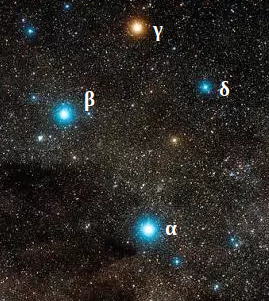
\includegraphics[width=0.25\textwidth]{crux_realphoto.png}
\caption{Foto asli rasi Crux. Oleh Eckhard Slawik.}
\label{fig:cruxasli}
\end{figure}

\begin{figure}[H]
\centering
%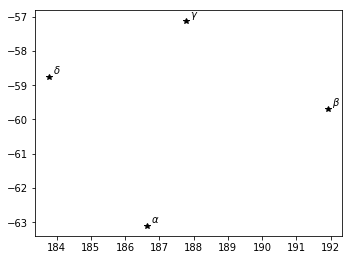
\includegraphics[width=0.49\textwidth]{crux_kartesian_RA_ke_kanan.png}
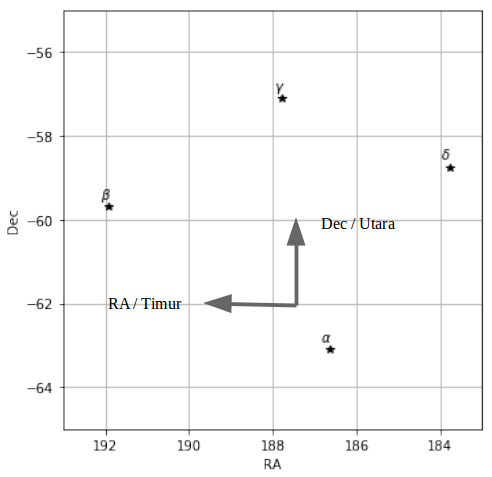
\includegraphics[scale=0.47]{crux_kartesian_RA_ke_kiri.png}
\caption{Plot dalam koordinat Kartesian dengan mimilih RA sebagai sumbu-$x$ dan deklinasi sebagai sumbu-$y$. Dalam kasus ini, untuk mendapatkan penampakan yang mirip dengan di langit, gunakanlah RA ke kiri, karena saat itu kita sedang melihat ke daerah langit selatan. Terlihat proporsinya jadi tidak mirip dengan yang terlihat di langit karena faktor proyeksi dari bentuk bola (3D) ke datar (2D), sama seperti masalah yang terjadi pada peta-datar Bumi yang kita jumpai. Untuk objek dekat ekuator masih akan mirip bentuknya, akan tetapi Crux yang dekat KLS akan terdeformasi jika kita plot dengan cara demikian. Bentuk Crux yang kita peroleh akan lebih mirip apabila kita gunakan koordinat polar atau jenis proyeksi yang lain.}
\label{fig:plotkartesian}
\end{figure}

\begin{figure}[H]
\centering
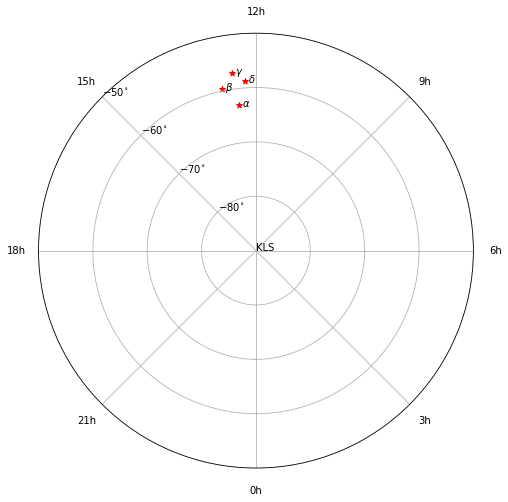
\includegraphics[width=0.65\textwidth]{crux_plot_polar.png}
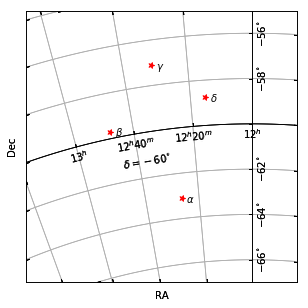
\includegraphics[width=0.5\textwidth]{crux_plot_polar_zoom.png}
\caption{Plot dalam koordinat polar. Plot dalam koordinat ini memberikan ``proyeksi'' yang lebih baik untuk menggambarkan ``bola'' langit ketimbang kartesian (bidang datar) biasa, sehingga bentuk Cruxnya lebih menyerupai yang kita lihat di langit. Pada plot ini, pusatnya adalah KLS, RA sebagai sudut putaran, dan deklinasi sebagai radius. Dapat dilihat bahwa apabila kita tarik garis dari $\gamma$Cru ke $\alpha$Cru, kita bisa peroleh arah KLS atau sebagai penanda arah Selatan.}
\label{fig:plotpolar}
\end{figure}

\item Berdasarkan sketsa pada poin (a), rangka layang-layang dibentuk oleh busur yang menghubungkan bintang $\alpha$ dan $\gamma$, serta $\beta$ dan $\delta$. Pada bola langit, buat sketsa segitiga bola yang menghubungkan antara KLS-$\alpha$-$\gamma$, dan KLS-$\beta$-$\delta$ (bisa juga dipilih KLU, sesuaikan saja hitungan matematikanya, karena secara geometri akan berbeda).

Dengan menggunakan aturan cosinus, dihitung:\\
Jarak antara $\alpha$-$\gamma$ (busur $s_1$)\\
\begin{eqnarray*}
\cos s_1&=&\cos (90\text{\degree}-|\delta_{\alpha}|)\cos (90\text{\degree}-|\delta_{\gamma}|)+\sin (90\text{\degree}-|\delta_{\alpha}|)\sin (90\text{\degree}-|\delta_{\gamma}|)\cos \Delta RA\\
\cos s_1&=&\sin |\delta_{\alpha}|\sin |\delta_{\gamma}|+\cos |\delta_{\alpha}|\cos |\delta_{\gamma}|\cos (RA_{\gamma}-RA_{\alpha})\\
\cos s_1&=&0,994\\
s_1&=&06\text{\degree}00\text{'}45\text{''}347
\end{eqnarray*}

Jarak antara $\beta$-$\delta$ (busur $s_2$)\\
\begin{eqnarray*}
\cos s_2&=&\cos (90\text{\degree}-|\delta_{\beta}|)\cos (90\text{\degree}-|\delta_{\delta}|)+\sin (90\text{\degree}-|\delta_{\beta}|)\sin (90\text{\degree}-|\delta_{\delta}|)\cos \Delta RA\\
\cos s_2&=&\sin |\delta_{\beta}|\sin |\delta_{\delta}|+\cos |\delta_{\beta}|\cos |\delta_{\delta}|\cos (RA_{\beta}-RA_{\delta})\\
\cos s_2&=&0,997\\
s_2&=&04\text{\degree}04\text{'}04\text{''}397
\end{eqnarray*}
Jadi, jarak sudut antar bintang yang membentuk rangka layang-layang adalah 06\degree 00'45''347 (antara $\alpha$ dan $\gamma$ Cru) dan 04\degree 04'04''397 (antara $\beta$ dan $\delta$ Cru).
\end{enumerate}


\question Di kutub Asteroid Ceres ditemukan bongkahan es. Es yang terakumulasi di Kutub diperkirakan meluncur ke lintang yang lebih rendah pada awal pembentukan asteroid. Akibat gravitasi Ceres yang kecil, bongkahan es lepas dan mengorbit permukaan asteroid. Anggaplah bongkahan es bermassa $m$ meluncur tanpa gesekan dan penguapan ke lintang yang lebih rendah akibat pengaruh gravitasi. Diketahui jejari rata-rata Ceres sebesar 473 km.
\begin{enumerate}[(a)]
\item Di lintang berapa bongkahan es lepas dari gravitasi Ceres?
\item Berapa jarak tempuh bongkahan es dari kutub hingga titik terakhir sebelum lepas ke orbit (dinyatakan dalam satuan km)
\item Berapa kecepatan bongkahan es saat lepas ke orbit (dinyatakan dalam satuan km/detik)
\end{enumerate}

\textit{Jawaban: }

Hmmmm... sepertinya kita diminta berimajinasi liar dalam soal ini. Kami tidak memahami maksud soalnya seperti apa. Sedikit yang terpikirkan:

\begin{enumerate}[(1).]
\item Kita asumsikan es meluncur/terpeleset secara alami dan perlahan akibat rotasi asteroid (gaya sentrifugal). Supaya hal itu terjadi sebetulnya perlu sedikit gaya gesek dan posisi awal bongkahan es tidak tepat persis di Kutub.

Untuk dapat mengorbit permukaan asteroid, maka bongkahan es harus memiliki kecepatan sebesar:
$$v=\sqrt{\frac{GM}{R}}$$
dengan $M$ adalah massa asteroid Ceres dan $R$ adalah radiusnya. 

Apabila kita andaikan kecepatan ini dicapai bongkahan es hanya dari gerak rotasi asteroid, maka kecepatan rotasi asteroid di ekuator harus lebih besar dari kecepatan ini. Jika kecepatan rotasi di ekuator asteroid lebih kecil dari nilai tersebut, maka bongkahan es tidak akan pernah lepas dari asteroid akibat gaya sentrifugal. Mengapa hal ini dapat terjadi? Karena apabila kecepatan itu tercapai, maka gaya gravitasi yang dirasakan bongkahan es akan sama besarnya dengan gaya sentrifugal, ingat:
\begin{eqnarray*}
m \cdot a_s &=& m \cdot g\\
m \cdot \frac{v^2}{R} &=& m \cdot \frac{GM}{R^2}
\end{eqnarray*}
yang apabila diteruskan akan kembali ke persamaan orbit lingkaran di atas. Sketsa gaya-gaya yang berlaku pada es di permukaan asteroid ditunjukkan oleh \autoref{fig:ceres}.

Jika kita gunakan cara ini maka ada beberapa komplikasi:
\begin{itemize}
\item Butuh data massa atau kerapatan Ceres
\item Butuh data periode
\item Secara fisis jika kecepatan rotasi asteroid Ceres lebih besar dari kecepatan suatu benda mengorbit di permukaan, maka ``kestabilan'' Ceres jadi dipertanyakan. Bisa jadi ia pecah karena rotasinya terlalu cepat. 
\end{itemize}
%v circular = 355.5 m/s
%v ekuator = 90.9787 m/s
\begin{figure}[H]
\centering
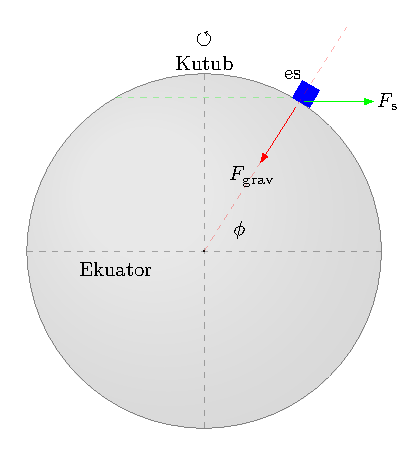
\includegraphics[width=0.4\textwidth]{ceres.pdf}
\caption{Sketsa es di permukaan Ceres yang berotasi kencang. $\phi$ menyatakan lintang tempat es berada saat mengalami gaya gravitasi sebesar $F_{\text{grav}}$ dan gaya sentrifugal $F_{\text{s}}$.}
\label{fig:ceres}
\end{figure}

\item Pemikiran lain misalnya saya bisa andaikan gravitasi yang di rasakan Ceres selalu mengarah ke ekuator. Layaknya bola yang berada di permukaan meja ``datar'' seperti pada \autoref{fig:ceres2}. Tentu hal ini tidak masuk akal, tetapi sepertinya mendekati yang dimaksud soal. Ceres tidak dianggap berotasi. Es jatuh/terpeleset murni akibat ``gravitasi aneh'' itu.
%\begin{figure}[H]
%\centering
%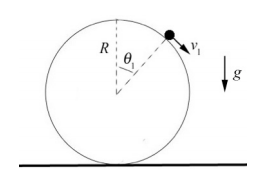
\includegraphics[width=0.5\textwidth]{ceres_g_flat.png}
%\caption{Sketsa es di permukaan Ceres, sedangkan Ceres berada di atas meja. Percepatan gravitasinya di anggap selalu mengarah ke ekuator/meja/``bawah''.}
%\label{fig:ceres2}
%\end{figure}
\begin{figure}[H]
\centering
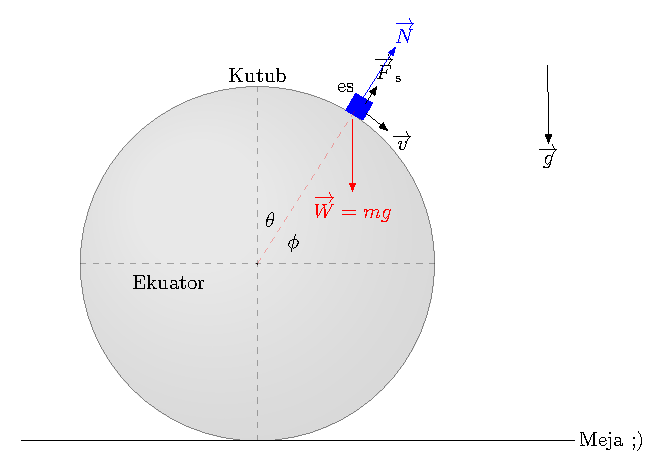
\includegraphics[width=0.65\textwidth]{ceres2.pdf}
\caption{Ceres tidak berputar dan gravitasi selalu mengarah ke ekuator.}
\label{fig:ceres2}
\end{figure}

Bongkahan es yang ada di Kutub sedikit bergeser, kemudian karena gravitasi ia `jatuh' ke ekuator. Karena $g$ mengarah ke ekuator/bawah/meja, maka akan ada saat di mana es lepas dari bola Ceres ini (lepas dari permukaan, bukan lepas dari gravitasi), yaitu ketika gaya normal yang di alaminya nol. Sehingga ketika es lepas berlaku hubungan:
\begin{eqnarray*}
N &=& mg \cos{\theta} - m \frac{v^2}{R}\\
0 &=& mg \cos{\theta_{\text{lepas}}} - m \frac{v_{\text{lepas}}^2}{R}\\
m \frac{v_{\text{lepas}}^2}{R} &=& mg \cos{\theta_{\text{lepas}}}
\end{eqnarray*}

Untuk masalah ini dapat kita gunakan hukum kekekalan energi. Jika kita ambil pusat bola Ceres sebagai acuan nol untuk menghitung energi potensial, maka:
\begin{eqnarray*}
E_{\text{awal}} &=& E_{\text{saat lepas}}\\
mgR &=& mgh_{\text{lepas}} + \frac{1}{2} m v_{\text{lepas}}^2\\
mgR &=& mgR\cos{\theta_{\text{lepas}}} + \frac{1}{2} mgR\cos{\theta_{\text{lepas}}}\\
1 &=& \frac{3}{2} \cos{\theta_{\text{lepas}}}\\
\cos{\theta_{\text{lepas}}} &=& \frac{2}{3}\\
\theta_{\text{lepas}} &=& 48,2^{\circ}
\end{eqnarray*}
Kecepatan saat lepas dapat dicari dengan memasukkan nilai $\cos$ ini ke persamaan sebelumnya,
\begin{eqnarray*}
m \frac{v_{\text{lepas}}^2}{R} &=& mg \cos{\theta_{\text{lepas}}}\\
v_{\text{lepas}}^2 &=& R \cdot g \cdot \frac{2}{3}\\
v_{\text{lepas}} &=& \sqrt{\frac{2}{3} g R}
\end{eqnarray*}

\begin{enumerate}[(a)]
\item Bongkahan es akan lepas di lintang $\phi_{\text{lepas}} = 90^{\circ} - \theta_{\text{lepas}} = 41,8^{\circ}$ 
\item Jarak yang ditempuh es dari Kutub sebelum lepas:
\begin{eqnarray*}
s &=& \theta_{\text{lepas, rad}} \cdot R\\
s &=& \frac{48,2}{360} \cdot 2 \pi \cdot R\\
s &=& 397,8 \text{  km} 
\end{eqnarray*}
\item Untuk menghitung kecepatan diperlukan nilai percepatan gravitasi $g$. Untuk itu kita bisa kira-kira nilai kerapatan Ceres $\rho = 2000$ kg/m$^3$ (kurang dari setengah kerapatan Bumi, $\rho_{\oplus} = 5500$ kg/m$^3$). Lalu kita hitung $g$ dipermukaan Ceres $ = \frac{GM}{R^2} = \frac{4}{3}G \pi \rho R = 0.264$ m/s$^2$.
\begin{equation*}
v_{\text{lepas}} = \sqrt{\frac{2}{3} \cdot 0.264 \cdot 473000} = 288.53 \text{  m/s} = 0.28853 \text{  km/s}
\end{equation*}
\end{enumerate}

\item Kita bisa asumsikan esnya ketabrak asteroid kecil, bisa langsung lepas ;)
\item Kita bisa asumsikan ada Saitama memukul batu esnya terlalu kencang, bisa langsung hancur ;))
\item dll.
\end{enumerate}




\question Saat energi potensial dan energi kinetik sama besar (energi total bernilai nol), sistem dikatakan pada keadaan kritis. Kerapatan alam semesta pada keadaan kritis, disebut kerapatan kritis, dapat diturunkan dari kekekalan energi Newton dengan bantuan rumus Hubble. Dengan asumsi alam semesta berbentuk bola, maka
\begin{enumerate}[(a)]
\item turunkanlah rumus kerapatan kritis yang bergantung pada konstanta Hubble dan konstanta gravitasi
\item hitunglah besar kerapatan kritis alam semesta
\item perkirakan jumlah seluruh bintang di alam semesta dengan asumsi seluruh massa materi yang menjadi bintang-bintang berasal dari 4\% kerapatan kritis, dan umur alam semesta 13 milyar tahun. Asumsikan pula bintang yang terbentuk berukuran sama dengan Matahari.
\end{enumerate}

\textit{Jawaban: }\\
\begin{enumerate}[(a)]
\item Secara sederhana, energi potensial gravitasi diri sendiri dan energi kinetik pengembangan alam semesta dapat dituliskan menjadi

\begin{eqnarray*}
E_k + E_p &=& 0 \\
\frac{1}{2} m v^2 - \frac{GMm}{R} &=& 0\\
\frac{GMm}{R} &=& \frac{1}{2} m v^2\\
\frac{GM}{R} &=& \frac{1}{2} v^2\\
\frac{G \frac{4}{3} \pi R^3 \rho_c}{ R } &=& \frac{1}{2} H_0^2 R^2\\
\frac{G 4 \pi \rho_c}{3} &=& \frac{1}{2} H_0^2\\
\rho_c &=& \frac{3 H_0^2}{8 \pi G}
\end{eqnarray*}

\item Besar kerapatan kritis alam semesta saat ini:

\begin{eqnarray*}
\rho_c &=& \frac{3 \cdot (69,3 \text{  km/s/Mpc})^2}{8 \cdot \pi \cdot 6,673 \times 10^{-11} \text{  m}^3/\text{kg}/\text{s}^2} \\
&=& \frac{3 \cdot (2,2458 \times 10^{-18} \text{  s}^{-1})^2}{8 \cdot \pi \cdot 6,673 \times 10^{-11} \text{  m}^3/\text{kg}/\text{s}^2}\\
&=& 9\times 10^{-27} \text{   kg/m}^3
\end{eqnarray*}

\item Massa total seluruh bintang di alam semesta (\textit{observable universe}):
\begin{eqnarray*}
M &=& 0,04 \cdot \rho_c \cdot V\\
&=& 0,04 \cdot 9\times 10^{-27} \cdot \frac{4}{3} \pi R^3\\
&=& 0,04 \cdot 9\times 10^{-27} \cdot \frac{4}{3} \pi \left((13 \times 10^9 \cdot 365,25 \cdot 24 \cdot 3600) \cdot 3 \times 10^8 \right)^3\\
&=& 2,811233 \times 10^{51} \text{  kg}\\
&=& 1,4 \times 10^{21} M_{\odot}
\end{eqnarray*}

Jadi, perkiraan jumlah bintang di alam semesta adalah $1,4 \times 10^{21}$ bintang.
\end{enumerate}




\question Supernova tipe Ia (SN Ia) merupakan salah satu objek paling terang di alam semesta. Magnitudo mutlak supernova tersebut dapat mencapai $M=-21$. Andaikan sebuah SN Ia tampak di galaksi M90 yang berada di Gugus Virgo. Galaksi M90 adalah sebuah galaksi spiral yang memiliki ukuran sumbu panjang sebesar 9,5 menit busur dan sumbu pendek 4,5 menit busur. Jika diketahui galaksi tersebut berada pada jarak 60 juta tahun cahaya dari Bumi dan memiliki kecerlangan permukaan sebesar 22 magnitudo per detik busur kuadrat, tentukan
\begin{enumerate}[(a)]
\item Manakah yang lebih terang, galaksi ataukah supernova? Buktikan jawaban kalian!
\item Hitunglah magnitudo semu gabungan dari galaksi M90 dan SN Ia!
\end{enumerate}

\textit{Jawaban: }

\begin{enumerate}[(a)]
\item Untuk mengetahui mana yang lebih terang, dapat kita bandingkan magnitudo mutlak kedua objek (atau magnitudo semunya, karena jaraknya sama).
\begin{itemize}
\item Luas galaksi M90 (luas elips) = $\pi a b = \pi \cdot (0,5 \cdot 9,5 \cdot 60) \cdot (0,5 \cdot 4,5 \cdot 60) = 120872,777$ detik busur kuadrat.

\item Jika M90 dianggap sebagai satu objek titik, maka magnitudonya dapat dicari dengan ``menjumlahkan'' fluks dari tiap detik busur kuadrat (mewakili total fluks),
\begin{eqnarray*}
m - m_s &=& -2,5 \log{\left(\frac{\text{area total}}{\text{area 1 detik busur kuadrat}}\right)}\\
m &=& m_s - 2,5 \log{\left(\text{area}\right)} \qquad \qquad \text{dengan  } m_s = \text{\textit{surface brightness}}\\
m &=& 22 - 2,5\log{(120872,777)} \\
m &=& 9,29418
\end{eqnarray*}

\item Magnitudo mutlak galaksi dapat dicari dari modulus jarak,
\begin{eqnarray*}
m - M &=& -5 + 5 \log{d}\\
M &=& 9,29418 + 5 - 5\log{\left(\frac{60 \times 10^6 \cdot 0.9461\times 10^{16}}{3.0857 \times 10^{16}} \text{ pc} \right)}\\
M &=& -22,03
\end{eqnarray*}

\end{itemize}
Ternyata dalam kasus ini galaksinya lebih terang dari supernova tersebut.

\item Magnitudo semu supernova di jarak tersebut dapat dicari terlebih dahulu,
\begin{eqnarray*}
m - M &=& -5 + 5 \log{d}\\
m &=& M -5 +5\log{d}\\
m &=& -21 - 5 + 5 \log{\left(\frac{60 \times 10^6 \cdot 0.9461\times 10^{16}}{3.0857 \times 10^{16}} \text{ pc} \right)}\\
m &=& 10,32
\end{eqnarray*}

Perbandingan fluks kedua objek,
\begin{eqnarray*}
m_{M90} - m_{SN} &=& -2,5 \log{\frac{E_{M90}}{E_{SN}}}\\
\frac{E_{M90}}{E_{SN}} &=& 10^{\frac{9,29418 - 10,32}{-2,5}}\\
\frac{E_{M90}}{E_{SN}} &=& 2,572338
\end{eqnarray*}

Magnitudo semu total gabungan kedua objek,
\begin{eqnarray*}
m_{tot} - m_{SN} &=& -2,5 \log{\frac{E_{M90} + E_{SN}}{E_{SN}}}\\
m_{tot} &=& m_{SN} -2,5 \log{\left(\frac{E_{M90}}{E_{SN}} + 1 \right)}\\
m_{tot} &=& 10,32 -2,5 \log{(2,572338 + 1)}\\
m_{tot} &=& 8,9376
\end{eqnarray*}

Magnitudo total gabungan galaksi dan supernovanya = 8,9376.

\end{enumerate}


\question Bintang Arcturus ($\alpha$ Bootes) dan Hadar ($\beta$ Centauri) masing-masing memiliki koordinat $\alpha_{\text{Arcturus}}=14,0$ jam, $\delta_{\text{Arcturus}}=+19^{\circ}$ dan $\alpha_{\text{Hadar}}=14,0$ jam, $\delta_{\text{Hadar}}=-60^{\circ}$
\begin{enumerate}[(a)]
\item Gambarkan posisi Arcturus dan Hadar pada bola langit.
\item Tentukan rentang lintang pengamat yang dapat mengamati kedua bintang tersebut secara bersamaan.
\end{enumerate}

\textit{Jawaban: }

\begin{enumerate}[(a)]
\item Posisi Arcturus dan Hadar di bola langit dapat digambarkan dengan terlebih dahulu memilih lintang pengamat dan posisi titik Aries (terserah kita). Misal paling gampang kita ambil pengamat di ekuator atau di Kutub Utara seperti pada \autoref{posisipengamat}. Yang paling penting adalah bagaimana kita menempatkan kutub langit, ekuator langit, bintang, dan titik Aries sehingga dapat menunjukkan koordinat bintang dengan benar.

\begin{figure}[H]
\centering
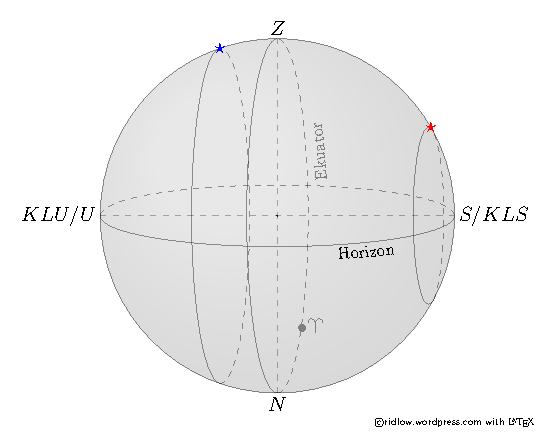
\includegraphics[width=0.54\textwidth]{nomor20_eq.pdf}
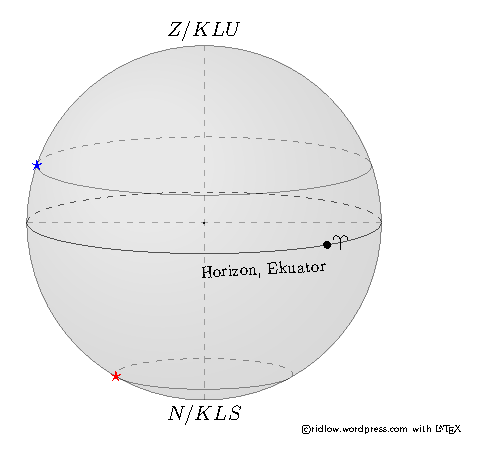
\includegraphics[width=0.45\textwidth]{nomor20_NorthPole.pdf}
\caption{Langit untuk pengamat di ekuator (kiri) dan kutub utara (kanan). Bintang Arcturus ($\alpha$ Bootes) dan Hadar ($\beta$ Centauri) masing-masing ditunjukkan dengan warna biru dan merah. Ditunjukkan pula lingkaran ekuator langit dan garis edar masing-masing bintang di langit.}
\label{posisipengamat}
\end{figure}

\item Pertanyaan (a) dan (b) dapat sebetulnya dijawab sekaligus dengan sketsa seperti pada \autoref{posisibintang}. Agar kedua bintang dapat diamati bersamaan, ketika satu bintang ada di atas horizon, bintang lain setidaknya harus sedang ada di horizon. Batas lintang paling utara yang dapat mengalami hal ini digambarkan oleh \autoref{posisibintang} bagian kiri, sedangkan batas lintang paling selatan yang dapat mengalami hal ini digambarkan oleh \autoref{posisibintang} bagian kanan. Dengan melihat sketsa bola langit tersebut, batas lintang paling utara dapat dihitung sebagai berikut.
\begin{eqnarray*}
|\delta_{Hadar}|+\phi_{1}&=&90\textbf{\degree}\\
60\text{\degree}+\phi_{1}&=&90\text{\degree}\\
\phi_{1}&=&30\text{\degree}
\end{eqnarray*}

Batas paling selatan dapat dihitung sebagai berikut.
\begin{eqnarray*}
|\delta_{Arcturus}|+\phi_{2}&=&90\textbf{\degree}\\
19\text{\degree}+\phi_{2}&=&90\text{\degree}\\
\phi_{2}&=&71\text{\degree}
\end{eqnarray*}

Jadi, rentang lintang pengamat yang dapat mengamati kedua bintang tersebut bersamaan di langit adalah 30\degree LU - 71\degree LS.

\begin{figure}[H]
\centering
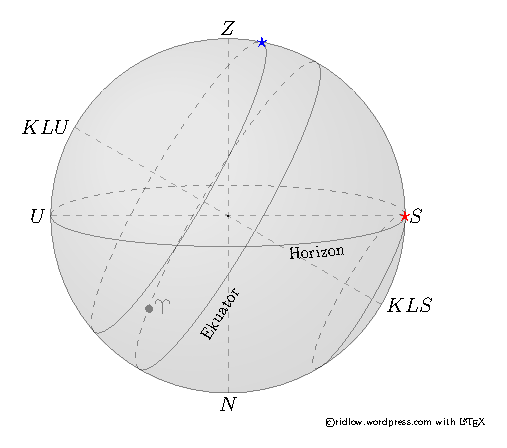
\includegraphics[width=0.49\textwidth]{nomor20_30LU.pdf}
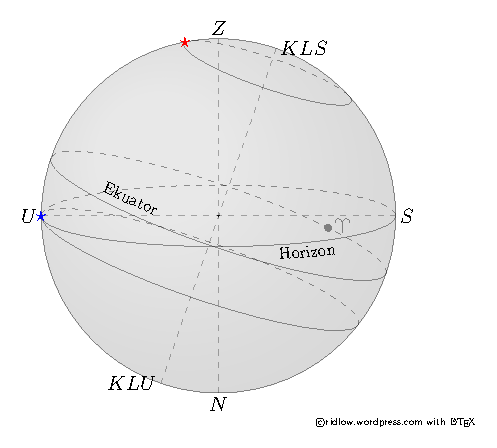
\includegraphics[width=0.49\textwidth]{nomor20_71LS.pdf}
\caption{Langit untuk pengamat di lintang $\phi_1^{\circ}$ LU (kiri) dan $\phi_2^{\circ}$ LS (kanan). Bintang Arcturus ($\alpha$ Bootes) dan Hadar ($\beta$ Centauri) yang sedang berada di meridian pengamat masing-masing ditunjukkan dengan warna biru dan merah. Ditunjukkan pula lingkaran ekuator langit dan garis edar masing-masing bintang di langit.}
\label{posisibintang}
\end{figure}

\end{enumerate}

\end{questions}

%\centering{\--- SOAL SELESAI\---}

\vspace{3cm}
\begin{flushright}
Solusi seperti ini dapat diperoleh di \url{http://ridlow.wordpress.com}
\end{flushright}
\end{document}
